\documentclass[tikz,border=6pt]{standalone}
\usepackage{amsmath}
\usepackage{newtxtext,newtxmath}
\usetikzlibrary{arrows.meta,calc}

\begin{document}
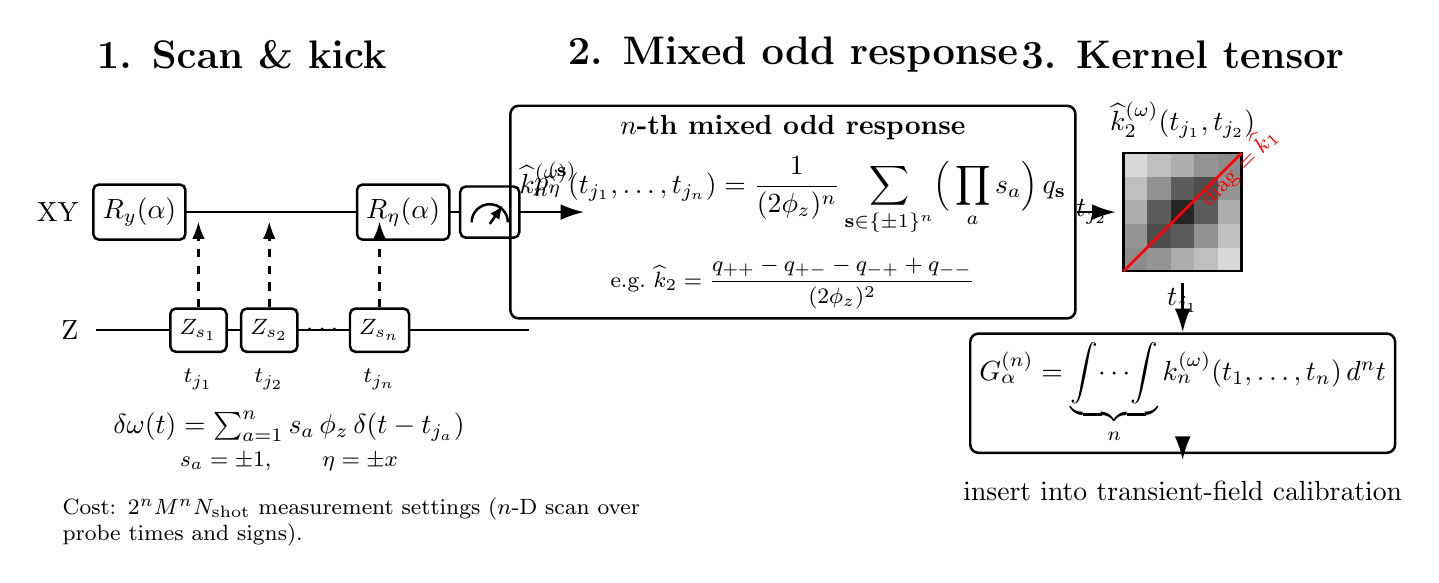
\begin{tikzpicture}[
  x=1cm,
  y=1cm,
  >=Latex,
  font=\large,
  line/.style={draw=black,line width=0.9pt},
  arrow/.style={line,-{Latex[length=3mm,width=2mm]}},
  block/.style={line,rounded corners=3pt,align=center,minimum height=0.8cm},
  gate/.style={line,fill=white,rounded corners=2pt,align=center,
               minimum width=0.95cm,minimum height=0.7cm,font=\normalsize},
  extractbox/.style={line,rounded corners=3pt,align=center,minimum width=5.6cm,minimum height=2.6cm,font=\normalsize},
  kick/.style={line,dashed,-{Latex[length=2.2mm,width=1.6mm]}}
]

% ---------------------------------------------------------------- headings
\node[font=\bfseries\Large] at (2.50,2.95) {1. Scan \& kick};
\node[font=\bfseries\Large] at (9.50,2.95) {2. Mixed odd response};
\node[font=\bfseries\Large] at (14.45,2.95) {3. Kernel tensor};

% ---------------------------------------------------------------- 1. dual-rail circuit (XY + Z)
% rail labels
\node[font=\normalsize,anchor=east] at (0.55,0.95) {XY};
\node[font=\normalsize,anchor=east] at (0.55,-0.55) {Z};

% XY rail: Ramsey with no free evolution (R_y and R_eta bracket the kick window)
\draw[line] (0.65,0.95) -- (6.15,0.95);
\node[gate] (ry)   at (1.20,0.95) {$R_y(\alpha)$};
\node[gate] (reta) at (4.55,0.95) {$R_\eta(\alpha)$};
% measurement meter symbol (standard quantum-circuit readout)
\node[gate,minimum width=0.75cm,minimum height=0.65cm] (meas) at (5.65,0.95) {};
\draw[line] (5.42,0.82) arc (180:0:0.23);
\draw[line,-{Latex[length=1.8mm,width=1.4mm]}] (5.65,0.80) -- (5.82,1.04);

% Z rail: virtual-Z sampling, all n kicks listed with an ellipsis
\draw[line] (0.65,-0.55) -- (6.15,-0.55);
\node[gate,minimum width=0.62cm,minimum height=0.55cm,font=\footnotesize] (z1) at (1.95,-0.55) {$Z_{s_1}$};
\node[gate,minimum width=0.62cm,minimum height=0.55cm,font=\footnotesize] (z2) at (2.85,-0.55) {$Z_{s_2}$};
\node[font=\normalsize] at (3.55,-0.55) {$\cdots$};
\node[gate,minimum width=0.62cm,minimum height=0.55cm,font=\footnotesize] (zn) at (4.25,-0.55) {$Z_{s_n}$};
% time ticks under the Z rail
\node[font=\footnotesize,anchor=north] at (1.95,-0.92) {$t_{j_1}$};
\node[font=\footnotesize,anchor=north] at (2.85,-0.92) {$t_{j_2}$};
\node[font=\footnotesize,anchor=north] at (4.25,-0.92) {$t_{j_n}$};
% dashed connectors: each virtual-Z kicks the qubit phase on the XY rail
\draw[kick] (z1.north) -- (1.95,0.83);
\draw[kick] (z2.north) -- (2.85,0.83);
\draw[kick] (zn.north) -- (4.25,0.83);

% physical content of the kicks + folded scan parameters
\node[font=\normalsize,anchor=north] at (3.10,-1.45)
  {$\delta\omega(t)=\textstyle\sum_{a=1}^{n}s_a\,\phi_z\,\delta(t-t_{j_a})$};
\node[font=\footnotesize,anchor=north] at (3.10,-1.98)
  {$s_a=\pm1,\qquad \eta=\pm x$};

\draw[arrow] (meas.east) -- node[above,font=\normalsize,pos=0.55,yshift=0.05cm]
  {$p_{\eta}^{(\mathbf{s})}$} (6.85,0.95);

% ---------------------------------------------------------------- 2. mixed odd response
\node[extractbox] (extract) at (9.50,0.95)
  {\textbf{$n$-th mixed odd response}\\[0.18cm]
   $\widehat{k}_n^{(\omega)}(t_{j_1},\dots,t_{j_n})=
   \dfrac{1}{(2\phi_z)^{n}}\displaystyle\sum_{\mathbf{s}\in\{\pm1\}^{n}}\!\Big(\prod_{a}s_a\Big)\,q_{\mathbf{s}}$\\[0.26cm]
   {\footnotesize e.g.\ $\widehat{k}_2=\dfrac{q_{++}-q_{+-}-q_{-+}+q_{--}}{(2\phi_z)^2}$}};

% ---------------------------------------------------------------- 3. kernel tensor + integral
\draw[arrow] (extract.east) -- (13.60,0.95);
\begin{scope}[shift={(13.70,0.20)}]
  \def\cs{0.30}
  \foreach \i in {0,...,4}{
    \foreach \k in {0,...,4}{
      \pgfmathsetmacro{\op}{min(1,0.55*exp(-0.16*((\i-2)^2+(\k-2)^2))+0.30*exp(-0.55*((\i-\k)^2)))}
      \fill[black,opacity=\op] (\i*\cs,\k*\cs) rectangle (\i*\cs+\cs,\k*\cs+\cs);
    }
  }
  \draw[line] (0,0) rectangle (5*\cs,5*\cs);
  \draw[red,line width=1pt] (0,0) -- (5*\cs,5*\cs);
  \node[font=\normalsize,anchor=north] at (2.5*\cs,-0.10) {$t_{j_1}$};
  \node[font=\normalsize,anchor=east] at (-0.08,2.5*\cs) {$t_{j_2}$};
  \node[font=\normalsize,anchor=south] at (2.5*\cs,5*\cs+0.06)
    {$\widehat{k}_2^{(\omega)}(t_{j_1},t_{j_2})$};
  \node[red,font=\footnotesize,anchor=west,rotate=45] at (3.05*\cs,2.65*\cs)
    {diag $=\widehat{k}_1$};
\end{scope}

\node[block,minimum width=4.6cm,minimum height=1.0cm,font=\normalsize] (area) at (14.45,-1.35)
  {$G_\alpha^{(n)}=\underbrace{\int\!\cdots\!\int}_{n}
   k_n^{(\omega)}(t_1,\dots,t_n)\,d^{n}t$};
\draw[arrow] (14.45,0.05) -- (area.north);
\draw[arrow] (area.south) -- (14.45,-2.20);
\node[font=\normalsize,align=center,anchor=north] at (14.45,-2.34)
  {insert into transient-field calibration};

% ---------------------------------------------------------------- cost (one line)
\node[font=\footnotesize,anchor=north west,text width=8.0cm] at (0.10,-2.55)
  {Cost: $2^{n} M^{n} N_{\mathrm{shot}}$ measurement settings ($n$-D scan over probe times and signs).};

\end{tikzpicture}
\end{document}
